\section{Barycentric coordinates}
Let us consider a triangle with top, bottom left and bottom right vertices to which we have assigned the colors red, green and blue respectively. The triangle barycentre divides each median into two parts that have a 2:1 ratio. \\
  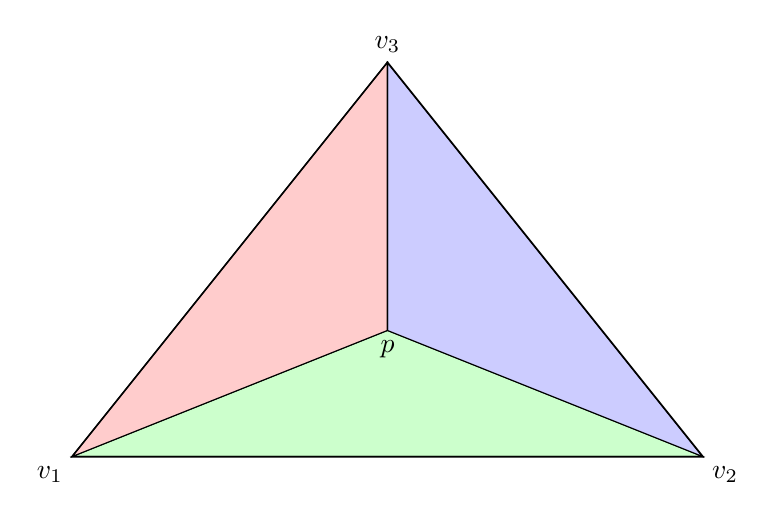
\begin{tikzpicture}
    \coordinate (L1) at (0,0);
    \coordinate (L2) at (8,0);
    \coordinate (L3) at (4,5);
    \coordinate (X) at (4,1.6);

    \draw[thick] (L1) -- coordinate[midway](md3) (L2)
                      -- coordinate[midway](md1) (L3)
                      -- coordinate[midway](md2) (L1) -- cycle;
    \filldraw[draw=black, fill=green!20] (L1) -- (X) -- (L2) -- cycle;
    \filldraw[draw=black, fill=red!20] (L1) -- (X) -- (L3) -- cycle;
    \filldraw[draw=black, fill=blue!20] (L3) -- (X) -- (L2) -- cycle;
    \draw (L1) node [below left] {$v_1$}
       -- (L2) node [below right] {$v_2$}
       -- (L3) node [above] {$v_3$}
       -- (X) node [below] {$p$};
    \end{tikzpicture}
    \\
    Let call the red area $w_1$, the blue green one $w_2$ and the blue one $w_3$. Normalazing each of them by the area of the triangle, we will get three values ($\lambda_1, \lambda_2, \lambda_3$) that are the barycentric coordinates of $p$ with respect to the triangle [$v_1, v_2, v_3$].
\\ \\ WRITE!!!!!!! introduction and all properties

\section{Linear Interpolation}
The standard linear interpolated visualisation is made passing three attributes (colors) for each vertex of a triangle. OpenGL will interpolate linearly the colors. That is possible thanks to the barycentric coordinates that will tell how much of each color is being mixed at any position.

\section{Flat Shading}

\section{Gouraud Shading}